\documentclass[a4paper]{article}
\usepackage[utf8]{inputenc}
\usepackage[russian]{babel}
\usepackage[T2]{fontenc}
\usepackage[warn]{mathtext}
\usepackage{graphicx}
\usepackage{amsmath}
\usepackage{floatflt}
\usepackage[left=20mm, top=20mm, right=20mm, bottom=20mm, footskip=10mm]{geometry}


\graphicspath{ {images/} }
\usepackage{multicol}
\setlength{\columnsep}{2cm}


\begin{document}

\begin{titlepage}
	\centering
	\vspace{5cm}
	{\scshape\LARGE Московский физико-технический институт \par}
	\vspace{5cm}

	{\huge\bfseries Газоразрядный стабилизатор напряжения \par}
	\vspace{1cm}
	{\scshape\Large Лабораторная работа по курсу <<Вакуумная электроника>>\par}
	\vspace{1cm}
	\vfill
\begin{flushright}
	{\large выполнила студентка 653 группы ФФКЭ}\par
	\vspace{0.3cm}
	{\LARGE Карпова Татьяна Кирилловна} \par

	
\end{flushright}
	

	\vfill

% Bottom of the page
	Долгопрудный, 2018 г.
\end{titlepage}

\section{Цель работы}
\begin{enumerate}
    \item Ознакомиться с основными особенностями тлеющего газового разряда и с основанным на его свойствах явлении стабилизации напряжения
\item Построить кривую зависимости напряжения зажигания от давления газа в стабиловольте (кривую Пашена) и определить минимальное значение напряжения.
\item Построить вольт-амперную характеристику газоразрядного стабилизатора напряжения.

\end{enumerate}

\section{Теоретические положения}

\textit{Газовым разрядом} в широком смысле называют всякое прохождение электрического тока
через газы. Газовые разряды бывают самостоятельные и несамостоятельные. \par 
Носители тока в \textit{несамостоятельном разряде} возникают за счёт внешней ионизации и с её
прекращением исчезают. При малых электрических полях плотность тока несамостоятельного разряда подчиняется дифференциальному закону Ома, так как концентрация ионизованных частиц (почти равная концентрации рекомбинирующих частиц) не зависит от внешнего поля E. При больших значениях поля все ионизованные частицы пролетят трубку, почти
не рекомбинируя с другими частицами, и ток выйдет на постоянную величину. Наконец,
при дальнейшем увеличении поля возникнет лавинообразное увеличение тока из-за того,
что заряженные частицы сами становятся способными вызвать ионизацию молекул за счёт
кинетической энергии, полученной или при движении в электрическом поле. \par
\textit{Самостоятельным разрядом} будем называть такой газовый разряд, в котором носители
тока возникают в результате тех процессов в газе, которые обусловлены приложенным к газу напряжением. Данный разряд продолжается и после прекращения действия ионизатора.
При лавинообразном несамостоятельном разряде положительные ионы могут выбить электроны из катода. Если в среднем из катода будет выбито более одного электрона, то заряд
можно считать самостоятельным. Количество необходимых для этого ионов зависит от давления и напряженности поля. Необходимое для этого напряжение называют \textit{напряжением
зажигания $U$з}. Напряжение зажигания и величина произведения давления газа на расстояние между электродами находятся в неявной зависимости, описываемой \textit{кривой Пашена}(см. рис. 1). При дальнейшем увеличении напряжения возникают тлеющий и дуговой разряды. \par

Работа газоразрядного стабилизатора напряжения  \textit{(стабилитрона)} основана на свойстве тлеющего разряда не изменять падение напряжения между электродами при изменении тока. Конструктивно стабилитрон состоит из двух коаксиальных электродов (катод обычно снаружи), помещённых в стеклянный или металлический баллон, содержащий смесь газов (как правило, инертных) при давлении в десятки торр. Рост тока при тлеющем разряде при таком расположении электродов происходит за счёт увеличения площади катода, охваченной разрядом, при этом плотность тока в ионизированной части газа остаётся неизменной, следовательно, остаётся неизменным и падение напряжения на разрядном промежутке. 

\begin{figure}[h]
\begin{center}
\begin{minipage}[h]{0.4\linewidth}
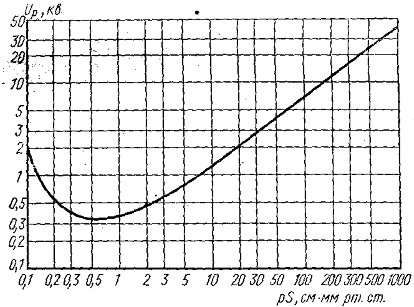
\includegraphics[width=1\linewidth]{pash.PNG}
\caption{Кривая Пашена} %% подпись к рисунку
\label{ris:experimoriginal} %% метка рисунка для ссылки на него
\end{minipage}
\hfill 
\begin{minipage}[h]{0.35\linewidth}
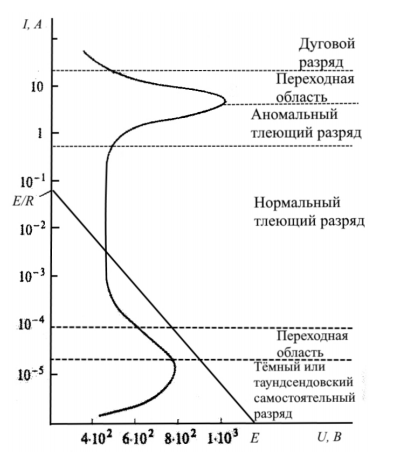
\includegraphics[width=1\linewidth]{va.PNG}
\caption{Вольт-амперная характеристика стабилитрона}
\label{ris:experimcoded}
\end{minipage}
\end{center}
\end{figure}

\section{Схема лабораторной установки}

Экспериментальная установка представляет собой стабиловольт, питающийся от источника. Стабиловольт находится при пониженном давлении (порядка 0.1 Торр), обеспечиваемом
форвакуумным насосом ФВ. Давление можно регулировать с помощью регулятора потока
FC и измеряется терморезистивным вакууметром VM. Напряжение и ток измеряются самим
источником. Принципиальная схема установки представлена на рис. 3, полная схема с указанием всех узлов и приборов - на рис. 4 (стабилитрон подключается к большой камере между кранов К2, К3, К4)

\begin{figure}[h]
\begin{center}
\begin{minipage}[h]{0.45\linewidth}
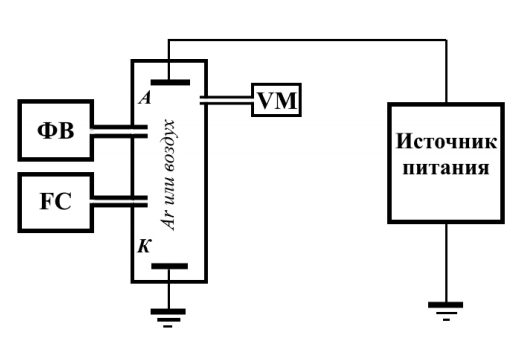
\includegraphics[width=1\linewidth]{setup.PNG}
\caption{Принципиальная схема установки} %% подпись к рисунку
\label{ris:experimoriginal} %% метка рисунка для ссылки на него
\end{minipage}
\hfill 
\begin{minipage}[h]{0.5\linewidth}
\includegraphics[width=1\linewidth]{facility.PNG}
\caption{Полная схема установки}
\label{ris:experimcoded}
\end{minipage}
\end{center}
\end{figure}


На схеме 4 обозначены: \\
$B_1$ - вакуумметр ёмкостной\\
$B_2$ - вакуумметр терморезисторный\\
$B_3$ - вакуумметр ионизационный\\
$K_1$ - кран турбомолекулярного насоса\\
$K_3$ - высоковакуумная заслонка\\
$K_4$ - форвакуумная заслонка\\
$K_2, K_7$ - коммутационные краны\\
Д - диафрагма\\
FC - регулятор газового потока (flow controller)\\
ТМН - турбомолекулярный насос\\
ФВН - форвакуумный насос\\

\section{Ход работы}

\subsection{Исследование кривой Пашена}

Снимем зависимость напряжения зажигания $U$з от давления в колбе стабилитрона P, измеренного с помощью терморезисторного вакуумметра. Для этого будем изменять значение натекания воздуха в систему ($Q_F_C$) и измерять напряжение, при котором в стабилитроне возникает газовый разряд. Результаты измерений запишем в таблицу 1 и графически представим на рисунке 5. Полученное минимальное значение зажигания для воздуха - 0.9 кВ. 

\begin{table}[h]
    \centering
    \begin{center}
    \caption{Зависимость напряжения зажигания от давления в системе}
        \label{tab:my_label}
    \end{center}
   \begin{tabular}{ |p{2cm}|p{2cm}|p{2cm}|  }

 \hline
 $Q_F_C, sccm$ & $P$, торр & $U$з, кВ   \\
\hline
\hline

100 & 1.7 & 1.42 \\
\hline
75 & 1.57 & 1.06 \\
\hline
50 & 1.4 & 0.81 \\
\hline
25 & 1.25 & 0.46 \\
\hline
10 & 1.07 & 0.23 \\
\hline
5 & 1.03 & 0.14 \\
\hline
1 & 2.4 & 0.05 \\
 \hline
\end{tabular}

\end{table}

\begin{figure}[h]
\begin{center}
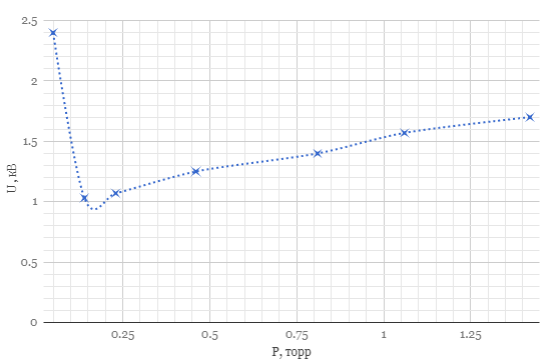
\includegraphics[width=13cm]{pashen.PNG}
\caption{Кривая Пашена для исследуемого стабилитрона}
\label{ris:experimoriginal} %% метка рисунка для ссылки на него

\end{center}
\end{figure}

Качественно поясним, почему кривая Пашена имеет минимум при некотором значении
$p_0d_0$. Заметим, что количество ионов $N_i$ в лавине, образованной одним электроном, при фиксированном напряжении на электродах $U$, при увеличении произведения $pd$ сначала увеличивается, а потом уменьшается. Увеличение $N_i$ при малых $pd$ связано с увеличением концентрации частиц и длины прибора. Уменьшение $N_i$ при больших значениях $pd$ происходит
из-за уменьшения поля E в трубке. Это приводит к тому, что на длине пробега электроны
приобретают меньшую энергию и ионизуют меньше частиц. Понятно, что оба эти фактора действуют при любых значениях $pd$, но в области малых значений определяющую роль
играет первый фактор, а при больших - второй. \par Наконец, вспомним, что напряжение зажигания $U$з - это такое напряжение, при котором лавина ионов, порождённая электроном,
выбьет один электрон из катода. Поскольку при фиксированном напряжении количество таких ионов сначала увеличивалось, а затем уменьшалось, $U$з должно сначала уменьшаться, а
потом увеличиваться, то есть проходить через минимум.

\subsection{Исследование вольт-амперной характеристики стабилитрона}

При постоянном значении натекания воздуха в систему снимем зависимость тока в цепи $I$ от напряжения зажигания $U$з. Результаты занесём в таблицу 2 и графически представим на рисунке 6. \par

При наших значениях тока ($\sim 10^{-3}$ А) и напряжения ($\sim 10^2 - 10^3$ В) вольт-амперная характеристика соответствует участку от нормального тлеющего разряда до переходной области. Характер зависимости $I(U)$, полученный нами в результате опыта, согласуется с представленным на рисунке 2. \par
Напряжение стабилизации для воздуха в результате опыта получилось равным 0.76 кВ

\begin{table}[h]
    \centering
    \begin{center}
    \caption{Зависимость напряжения зажигания от давления в системе}
        \label{tab:my_label}
    \end{center}
   \begin{tabular}{ |p{2cm}|p{2cm}||p{2cm}| p{2cm}| }

 \hline
 $U$з, кВ & $I$, А & $U$з, кВ & $I$, А   \\
\hline
\hline

0.75 & 1.98 & 0.83 & 1 \\
\hline
0.75 & 1.84 & 0.83 & 0.92\\
\hline
0.76 & 1.67 & 0.84 & 0.85\\
\hline
0.76 & 1.55 & 0.86 & 0.74\\
\hline
0.76 & 1.48 & 0.86 & 0.66\\
\hline
0.76 & 1.39 & 0.88 & 0.54\\
\hline
0.76 & 1.29 & 0.89 & 0.45\\
\hline
0.78 & 1.24 & 0.9 & 0.32\\
\hline
0.79 & 1.19 & 0.91 & 0.25\\
\hline
0.82 & 1.08 & 0.91 & 0.15\\
 \hline
\end{tabular}

\end{table}

\begin{figure}[h]
\begin{center}
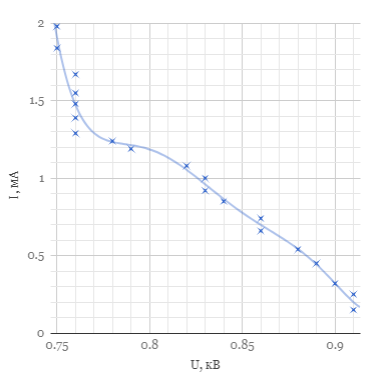
\includegraphics[width=10cm]{vach.PNG}
\caption{Вольт-амперная исследуемого стабилитрона}
\label{ris:experimoriginal} %% метка рисунка для ссылки на него

\end{center}
\end{figure}

\section{Вывод}
В ходе исследования газоразрядного стабилизатора напряжения были получены следующие результаты:

\begin{enumerate}
    \item Исследована природа газового разряда, разновидности газового разряда, принцип работы и основные характеристики стабилитрона (понятие кривой Пашена и вольт-амперная характеристика стабилитрона при широких диапазонах напряжения).
    \item Изучена кривая Пашена в ходе эксперимента (снята зависимость значения напряжения зажигания разряда от давления в колбе прибора), исследован характер этой зависимости и физические причины её нелинейности.
    \item Получена вольт-амперная характеристика прибора в режиме работы нормального тлеющего разряда и в переходной области, исследован характер зависимости $I(U)$ и проведено его сравнение с действительными характеристиками прибора.
\end{enumerate}

\end{document}
